\documentclass[tikz,border=10pt]{standalone}

\usepackage{xcolor}
\usetikzlibrary{arrows.meta,positioning}

\begin{document}

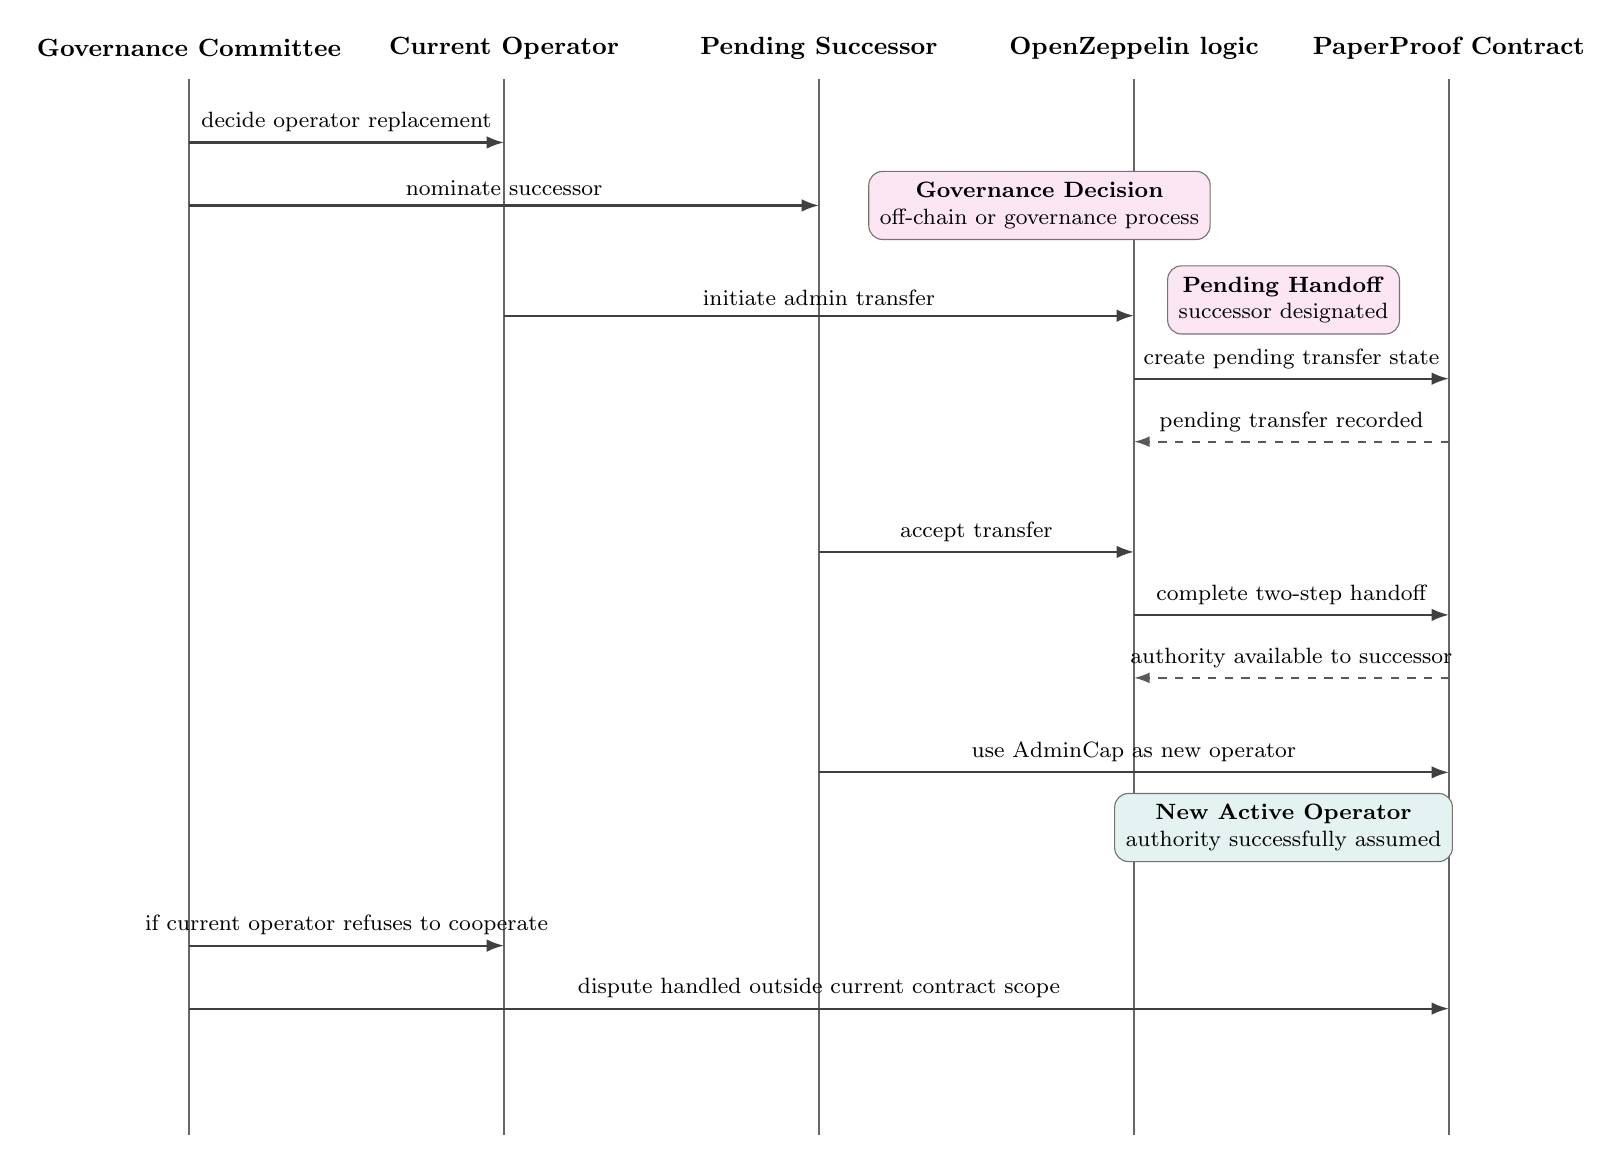
\begin{tikzpicture}[
    font=\small,
    lifeline/.style={draw=black!60, thick},
    msg/.style={-{Latex[length=2.2mm,width=1.6mm]}, thick, draw=black!75},
    reply/.style={-{Latex[length=2.0mm,width=1.4mm]}, thick, dashed, draw=black!65},
    note/.style={
        rectangle,
        rounded corners=4pt,
        draw=black!40,
        fill=gray!8,
        align=left,
        font=\footnotesize,
        inner sep=5pt
    },
    state/.style={
        rectangle,
        rounded corners=5pt,
        draw=black!55,
        fill=magenta!10,
        align=center,
        font=\footnotesize,
        inner sep=4pt
    }
]

% =========================================================
% Participants
% =========================================================
\node at (0,0) {\textbf{Governance Committee}};
\node at (4.0,0) {\textbf{Current Operator}};
\node at (8.0,0) {\textbf{Pending Successor}};
\node at (12.0,0) {\textbf{OpenZeppelin logic}};
\node at (16.0,0) {\textbf{PaperProof Contract}};

% Lifelines
\draw[lifeline] (0,-0.4) -- (0,-13.8);
\draw[lifeline] (4.0,-0.4) -- (4.0,-13.8);
\draw[lifeline] (8.0,-0.4) -- (8.0,-13.8);
\draw[lifeline] (12.0,-0.4) -- (12.0,-13.8);
\draw[lifeline] (16.0,-0.4) -- (16.0,-13.8);

% =========================================================
% Sequence messages
% =========================================================

% Committee decision
\draw[msg] (0,-1.2) -- node[above, font=\footnotesize] {decide operator replacement} (4.0,-1.2);
\draw[msg] (0,-2.0) -- node[above, font=\footnotesize] {nominate successor} (8.0,-2.0);

\node[state] at (10.8,-2.0) {\textbf{Governance Decision}\\off-chain or governance process};

% Initiate transfer
\draw[msg] (4.0,-3.4) -- node[above, font=\footnotesize] {initiate admin transfer} (12.0,-3.4);
\draw[msg] (12.0,-4.2) -- node[above, font=\footnotesize] {create pending transfer state} (16.0,-4.2);
\draw[reply] (16.0,-5.0) -- node[above, font=\footnotesize] {pending transfer recorded} (12.0,-5.0);

\node[state] at (13.9,-3.2) {\textbf{Pending Handoff}\\successor designated};

% Successor accepts
\draw[msg] (8.0,-6.4) -- node[above, font=\footnotesize] {accept transfer} (12.0,-6.4);
\draw[msg] (12.0,-7.2) -- node[above, font=\footnotesize] {complete two-step handoff} (16.0,-7.2);
\draw[reply] (16.0,-8.0) -- node[above, font=\footnotesize] {authority available to successor} (12.0,-8.0);

% New operator active
\draw[msg] (8.0,-9.2) -- node[above, font=\footnotesize] {use AdminCap as new operator} (16.0,-9.2);

\node[state, fill=teal!10] at (13.9,-9.9) {\textbf{New Active Operator}\\authority successfully assumed};

% Optional non-cooperative path
\draw[msg] (0,-11.4) -- node[above, font=\footnotesize] {if current operator refuses to cooperate} (4.0,-11.4);
\draw[msg] (0,-12.2) -- node[above, font=\footnotesize] {dispute handled outside current contract scope} (16.0,-12.2);

\end{tikzpicture}

\end{document}
